\documentclass{beamer}

\usepackage{amsfonts}
\usepackage{amsmath}
\usepackage{longtable}
\usepackage{csquotes}
\usepackage{standalone}

\usepackage{graphicx}
\graphicspath{{../pictures/}}

\usepackage{tikz}
\usetikzlibrary{shapes, calc, arrows, decorations.markings,
  decorations.pathmorphing, decorations, patterns, chains, snakes,
  backgrounds, positioning, fit, petri}
\newcommand{\inputpicture}[1]{\input{../drawings/#1}}

\usepackage{listings}
\lstset{language=C, basicstyle=\ttfamily, breaklines=true, keepspaces=true,
  keywordstyle=\color{blue}}

\usepackage{bytefield}

\usefonttheme{professionalfonts}
\usefonttheme{serif}
\usepackage{fontspec}
\setromanfont{CMU Serif}
\setsansfont{CMU Sans Serif}
\setmonofont{CMU Typewriter Text}

\usepackage{hyperref}
\hypersetup{colorlinks=true, linkcolor=black, filecolor=black, citecolor=black,
  urlcolor=blue , pdfauthor=Evgenii Iuliugin <yulyugin@gmail.com>,
  pdftitle=Fundamentals of Full-Platform Simulation}

\usepackage{underscore}
\usepackage{amsthm}

\subtitle{Fundamentals of Full-Platform Simulation}
\subject{Lecture}
\date{\today}

\author[Evgenii Iuliugin]{
  Evgenii Iuliugin \small{\href{mailto:yulyugin@gmail.com}{yulyugin@gmail.com}}}
\typeout{Copyright 2021 Evgenii Iuliugin}

\usetheme{Berlin}
\setbeamertemplate{navigation symbols}{}

\newcommand{\finalslide}{
    {\huge{Thank you!}\par}

    \vfill
    Slides and material are available at
    \url{https://github.com/yulyugin/sim-lectures}
    \vfill

    \tiny{\textit{Note}: All trademarks are the property of their respective
        owners.
        The presented point of view reflects the personal opinion of the author.

        %All the materials are licensed under the Creative Commons
        %Attribution-NonCommercial-ShareAlike 4.0 Worldwide. To view a copy of
        %this license, visit
        %\url{http://creativecommons.org/licenses/by-nc-sa/4.0/}.
    }
}


\title{Simulation of Architectural State}

\begin{document}

\startslides

\begin{frame}{On the Previous Lecture:}
\begin{itemize}
\item Full-Platform Simulation:
  \begin{itemize}
  \item Timer,
  \item Delay-Response Communication.
  \end{itemize}
\item Discrete Event Simulation (DES).
\item Co-Simulation: DES And Processor Models.
\item Multi-Processor Simulation.
\end{itemize}
\end{frame}

\begin{frame}{Questions}
\begin{itemize}
\item Can a processor be simulated using DES?\pause
\item What is dangerous about too large quantum in a multi-processor model?\pause
\item It it possible to have two event queues in a single simulation?
\end{itemize}
\end{frame}

\begin{frame}{Platform}
\centering
\vfill
\inputpicture{full-platform}
\vfill
\end{frame}

\section{Register File}

% TODO: Use RISC-V instead of OpenRISC.
\begin{frame}{Register File}
\centering
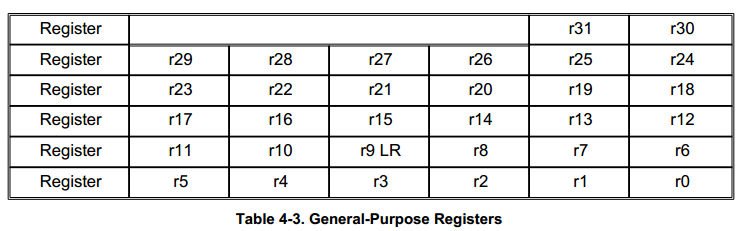
\includegraphics[width=0.8\textwidth]{or1k-gprs}

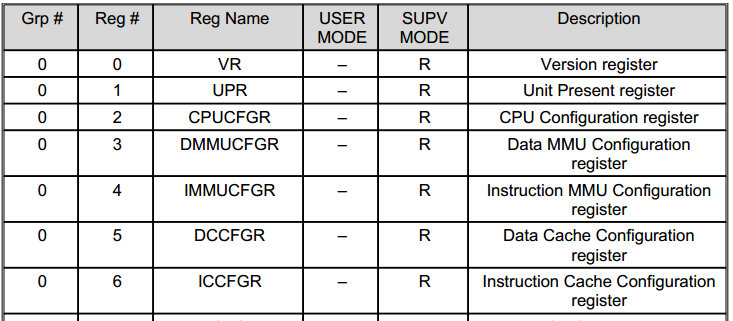
\includegraphics[width=0.8\textwidth]{or1k-sprs}

\tiny{OpenCores. OpenRISC 1000 Architecture Manual rev 1.0}
\end{frame}

\begin{frame}[fragile]{C-Structure}
\begin{lstlisting}
#include <stdint.h>

#define NO_GPRS 32
#define NO_SPRS 1024
#define REG_VR 0
#define REG_UPR 1

/* ... */

typedef struct cpu {
    uint32_t pc;
    uint32_t gprs[NO_GPRS];
    uint32_t sprs[NO_SPRS];
} cpu_t;
\end{lstlisting}
\end{frame}

\begin{frame}{Host Registers}
\begin{itemize}
\item Access to structure members in memory is slow.
\item Access to host registers is faster.
\item Put guest register in host registers.
\item \texttt{register cpu_t *cpu __asm__("rbp");}
\end{itemize}
\end{frame}

\begin{frame}{Host Registers}
\begin{itemize}
\item All guest registers may not fit host registers.
\item Put the most frequently used guest registers in host registers.
\item Simulator code becomes non-portable.
\item Special registers: \texttt{PC, SP, FP[0-7]}.
\item Interference with compiler: additional register pressure.
\end{itemize}
\end{frame}

\section{Lazy Calculations}

\begin{frame}{Lazy Calculations}
\begin{itemize}
\item Do not calculate state of a register until it is needed.
\item Example: Intel\reg~IA-32 \texttt{EFLAGS} register.
\item \texttt{flags = f(dst, src1, src2, op)} for the last instruction changing
  flags.
\end{itemize}
\vfill
\centering
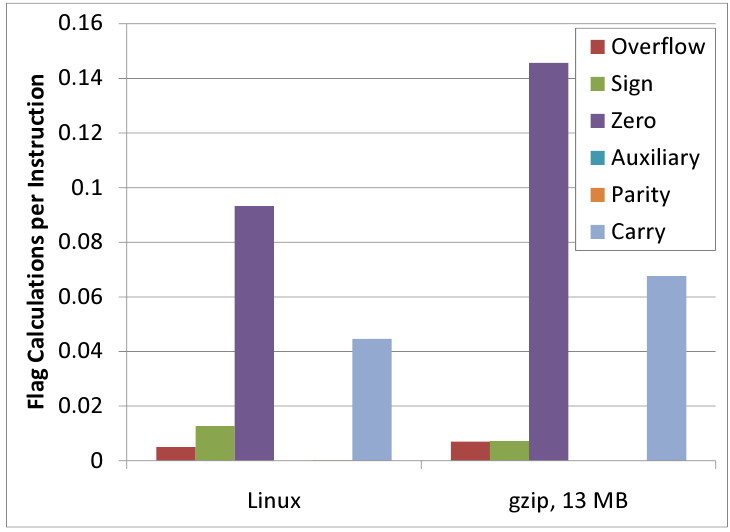
\includegraphics[width=0.5\textwidth]{lazy-eflags}

\tiny{Yair Lifshitz et al. Zsim: A Fast Architectural Simulator for ISA Design-Space Exploration}
\end{frame}

\section{Large Arrays}

\begin{frame}[fragile]{RAM And Other Large Array Accesses}
Allocate dynamic memory from the heap.
\vfill
\begin{lstlisting}
uint8_t *buf = (uint8_t *)calloc(BUF_SIZE, 1);

/* read */
uint8_t val = buf[offset];

/* write */
buf[offset] = val;
\end{lstlisting}
\vfill\pause
What to do if \texttt{BUF_SIZE} 16GB but host memory is only 4GB?
\end{frame}

\begin{frame}[fragile]{Lazy Memory Allocation}
For a continuous address range a storage can be allocated on demand in chunks
of a fixed size (pages).
\vfill
\begin{lstlisting}
page = addr & PAGE_MASK;
hptr = lookup_hptr(page);
if (!hptr)
    hptr = allocate_hptr(page);
assert(hptr);
haddr = hptr + (addr & PAGE_OFFSET);
\end{lstlisting}
\vfill
Swap <<old>> pages out to disk If memory is insufficient
\end{frame}

\begin{frame}[fragile]{Does It Sound Familiar?}
\begin{itemize}
\item It's a virtual memory!
\item POSIX-systems have \texttt{mmap()} mechanism.
\end{itemize}
\vfill
\begin{lstlisting}
void *mmap(void *addr, size_t len, int prot,
           int flags, int fildes, off_t off); 
\end{lstlisting}
\vfill
\centering
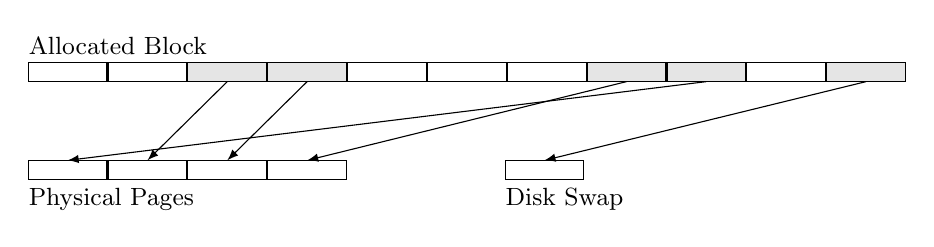
\begin{tikzpicture}[>=latex, font=\small, node distance=0mm, inner xsep=0pt, text width = 10mm, every node/.style=draw]
\begin{scope}[start chain]
    \node [on chain] (vp0) {};
    \node [on chain] {};
    \node [fill=black!10, on chain] (vp2) {};
    \node [fill=black!10, on chain] (vp3) {};
    \node [on chain] {};
    \node [on chain] {};
    \node [on chain] {};    
    \node [fill=black!10, on chain] (vp4) {};    
    \node [fill=black!10, on chain] (vp1) {};    
    \node [on chain] {};    
    \node [fill=black!10, on chain] (vp5) {};    
\end{scope}

\begin{scope}[start chain]
    \node [on chain, below=1cm of vp0] (pp1) {} ;
    \node [on chain] (pp2) {};
    \node [on chain] (pp3) {};
    \node [on chain] (pp4) {};

\end{scope}
    \node [right=2cm of pp4] (dp1) {};    

\draw[->] (vp1.south) -- (pp1.north);
\draw[->] (vp2.south) -- (pp2.north);
\draw[->] (vp3.south) -- (pp3.north);
\draw[->] (vp4.south) -- (pp4.north);
\draw[->] (vp5.south) -- (dp1.north);
    
\node[draw=none, above=0.1cm of vp0.east, text width=4cm, xshift=1cm] {Allocated Block};
\node[draw=none, below=0.1cm of pp1.east, text width=4cm, xshift=1cm] {Physical Pages};
\node[draw=none, below=0.1cm of dp1.east, text width=4cm, xshift=1cm] {Disk Swap};
\end{tikzpicture}
\end{frame}

\section{Register, Fields, Banks}

\begin{frame}[fragile]{Two Ways to Interact With Platform Registers}
\begin{enumerate}
\item
Programmable I/O (PIO) --- specific processor instructions to communicate with
peripheral devices (Intel\reg~IA-32, IBM s390, PDP-8).
\vfill
\begin{verbatim}
IN EAX, DX
OUT DX, EAX
\end{verbatim}
\vfill\pause
\item
Memory mapped I/O (MMIO) --- unified approach to access RAM and devices
(Intel\reg~IA-32, ADM, PDP-11).
\vfill
\begin{verbatim}
MOV [mem], reg
MOV reg, [mem]
\end{verbatim}
\end{enumerate}
\end{frame}

\begin{frame}{Operations on Registers}
\begin{itemize}
\item Read, write, fetch, prefetch.
\item Storage (<<dummy>>) registers and registers with side-effects.
\item Types of register accesses:
\begin{itemize}
\item Read-Write (RW) --- control and status registers,
\item Write (WO) --- command registers,
\item Read (R) --- info registers,
\item Inquiry --- <<invisible>> non-architectural access without side effects,
\item Reset.
\end{itemize}
\end{itemize}
\end{frame}

\begin{frame}[fragile]{Operations on Registers}
\begin{lstlisting}[basicstyle=\small]
template <class rtype> class IRegister {
    virtual Exception Read(rtype& retval) = 0;
    virtual Exception Fetch(rtype& retval) = 0;
    virtual Exception Prefetch(rtype& retval) = 0;
    virtual Exception Write(const rtype& newval) = 0;
    virtual bool InquiryRead(rtype& retval) = 0;
    virtual bool InquiryWrite(const rtype& newval) = 0;
    virtual void Reset() = 0;
};
\end{lstlisting}
\end{frame}

\begin{frame}[fragile]{Bit Fields}
\centering
\begin{bytefield}[bitwidth=0.8em, endianness=big]{32}
\bitheader{31,19,18,17,16,15,13,12,11,8,7,0} \\
\bitbox{13}{}&\bitbox{2}{\tiny{mode}} & \bitbox{1}{\rotatebox{90}{\tiny{mask}}} & \bitbox{3}{} & \bitbox{1}{\rotatebox{90}{\tiny{status}}} & \bitbox{4}{} & \bitbox{8}{vector} \\
\end{bytefield}

\tiny{APIC LVT Timer. Intel\reg 64 and IA-32 Architectures Software Developer’s Manual}
\vfill
\normalsize
\begin{itemize}
\item Real basic unit in specification and simulation.
\item May have completely different properties in one register.
\end{itemize}
\end{frame}

\begin{frame}[fragile]{Register Banks}
Register Bank --- group of device register located in the same area.
Can be viewed as hardware equivalent of a software array.
\vfill
\centering
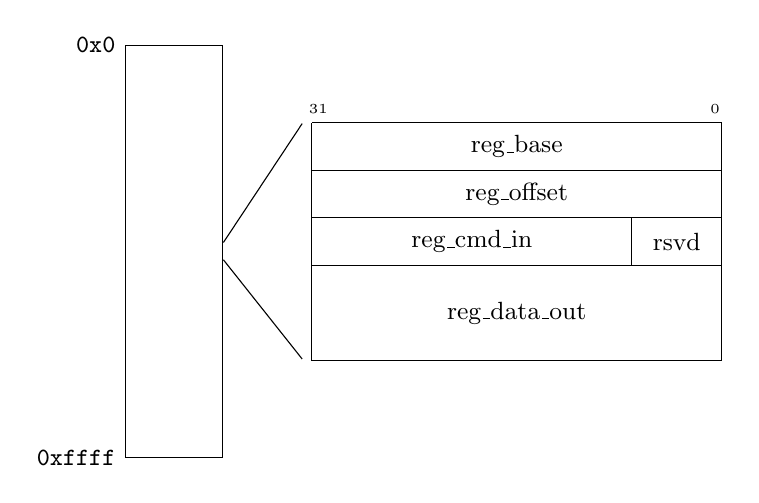
\begin{tikzpicture}[font=\small, >=latex]

\node[text height=5cm, text width=1cm, draw] (physspace) {};

\node[right=of physspace] (bank) {
\begin{bytefield}[bitwidth=.5em, endianness=big]{32}
\bitheader{31, 0}\\
\wordbox{1}{reg_base}\\
\wordbox{1}{reg_offset}\\
\bitbox{25}{reg_cmd_in} & \bitbox{7}{rsvd}\\
\wordbox{2}{reg_data_out}\\
\end{bytefield}
};

\draw (physspace.10) -- ([yshift=-0.25cm]bank.north west);
\draw (physspace.350) -- ([yshift=0.5cm]bank.south west);

\node[left=0cm of physspace.north west] {\texttt{0x0}};
\node[left=0cm of physspace.south west] {\texttt{0xffff}};

\end{tikzpicture}
\end{frame}

\begin{frame}{Memory Maps}
\centering
\inputpicture{memmap}
\end{frame}

\begin{frame}{Example: devmgmt.msc}
\centering
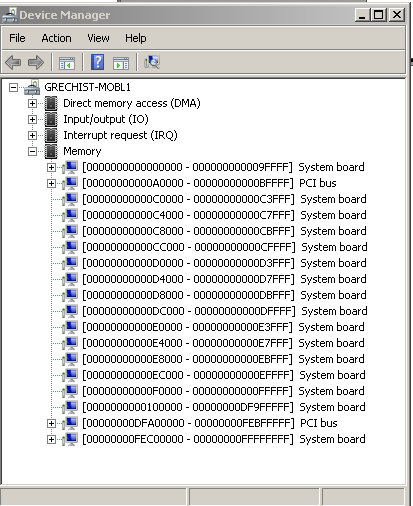
\includegraphics[width=0.8\textwidth]{devicemanager}
\end{frame}

\section{Address Translation}

\begin{frame}{Address Translation}
\begin{itemize}
\item Real system: \textbf{virtual} to \textbf{physical}.
\item[] \pause
\item Simulated system: \textbf{guest virtual} to \textbf{guest physical}.\pause
\item Simulator: \textbf{guest physical} to \textbf{host virtual}.\pause
\item Host OS: \textbf{host virtual} to \textbf{host physical}.\pause
\end{itemize}
\end{frame}

\begin{frame}{Optimization for Address Translation}
\begin{itemize}
\item \texttt{gv2gp + gp2hv + hv2hp}.\pause
\item Caching on all levels:
\begin{itemize}
\item \texttt{hv2hp} caching is done by host TLB.
\item Other are handled by software TLB-like cache.\pause
\end{itemize}
\item More?\pause
\item \texttt{gv2gp + gp2hv + hv2hp = gv2hv + hv2hp}.
\item \texttt{gv2hv} often referred as \texttt{v2h}. Cache \texttt{v2h}.\pause
\item More?\pause
\item Cache \texttt{gv2hp} --- hardware virtualization.
\end{itemize}
\end{frame}

\section{Endianness}

\begin{frame}{Bit, Byte, Word}
\begin{itemize}
\item Bit (binary digital) \pause --- the most basic unit of information.
  Bit represents logical state with two possible values: usually '1'/'0' or
  'true'/'false'.
\item Byte \pause --- smallest addressable unit of memory in a particular
  architecture.\pause
\item Octet \pause --- a unit of digital information containing 8 bits.\pause
\item Word (a.k.a. machine word) \pause --- a unit of information that can be
  handled at once by a particular CPU architecture.
\end{itemize}
\pause\vfill
Intel: byte --- 8 bit, word --- 16 bit, dword --- 32 bit, qword --- 64 bit.
\end{frame}

\begin{frame}{Endianness --- Order of Bytes}
\begin{columns}[onlytextwidth]
\begin{column}{0.5\textwidth}
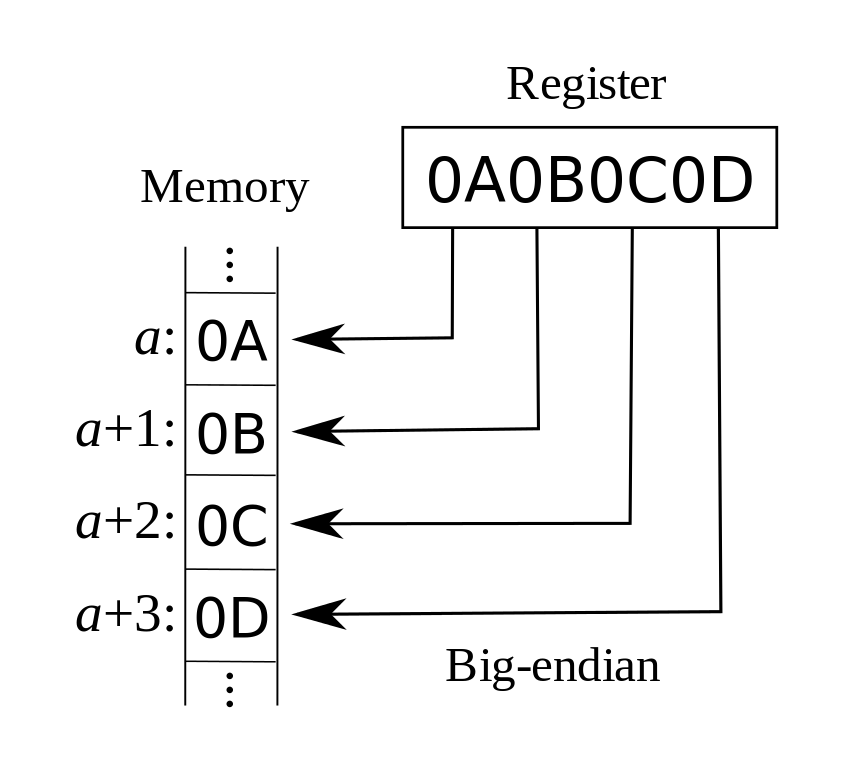
\includegraphics[width=\textwidth]{./be}
\end{column}

\begin{column}{0.5\textwidth}
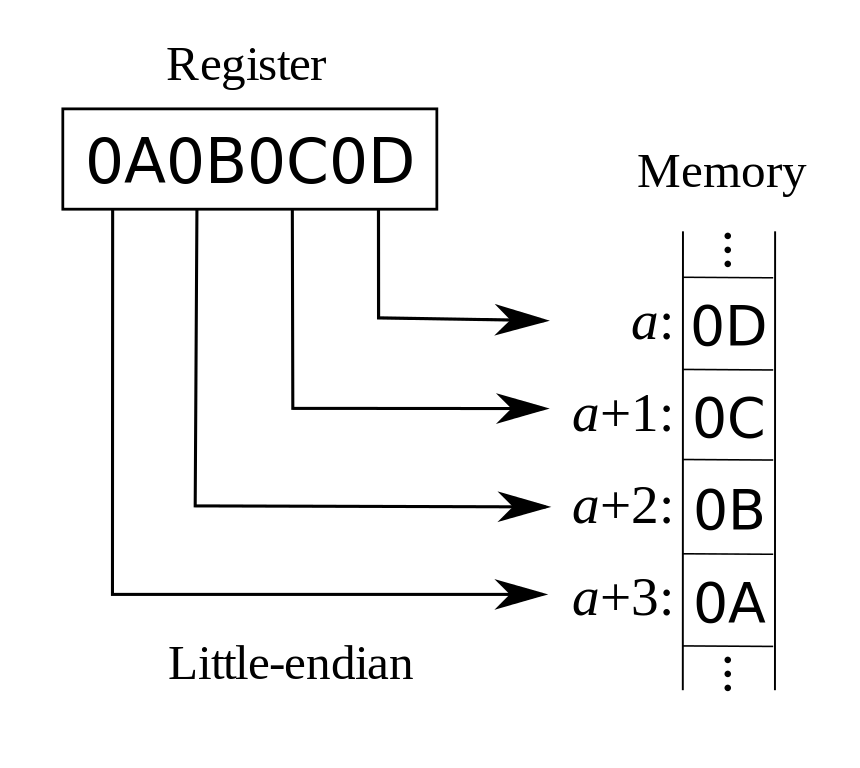
\includegraphics[width=\textwidth]{./le}
\end{column}
\end{columns}
\end{frame}

\begin{frame}{Endianness --- Order of Bytes}
\begin{itemize}
\item \textbf{Big-endian (BE)} stores \textit{most} significant byte of a
  word at the smallest address.
\item \textbf{Little-endian (LE)} stores \textit{least} significant byte of a
  word at the smallest address.\pause
\item \textbf{Middle-endian} or \textbf{mixed-endian} --- numerous other
  orderings.\pause
\item \textbf{Bi-endianness} --- architectural feature allowing switchable
  endianness.
\end{itemize}
\end{frame}

\begin{frame}{Endianness --- Examples}
\begin{itemize}
\item Big-endian: SPARC, IBM z/Architecture, OpenRISC\dots
\item Little-endian: Intel\reg IA-32, AMD64, Nios II\dots
\item Bi-endian: ARM, Power ISA, Intel\reg IA-64, RISC-V\dots
\end{itemize}
\end{frame}

\section*{Conclusions}

\begin{frame}[allowframebreaks]{Bibliography}
\begin{thebibliography}{99}
\bibitem{} \textit{Y. Lifshitz, R. Cohn, I. Livni, O. Tabach, M. Charney, K.
  Hazelwood}. Zsim: A Fast Architectural Simulator for ISA Design-Space
  Exploration.
\bibitem{} \textit{S.~Shwartsman, D.~Mihoka}. How Bochs Works Under the Hood.
  2nd edition.
\bibitem{} \textit{M. Domeika, M. Loenko, P. Ozhdikhin, E. Brevnov}. Bi-Endian
  Compiler: A Robust and High Performance Approach for Migrating Byte Order
  Sensitive Applications.
\end{thebibliography}
\end{frame}

\begin{frame}{On the Next Lecture:}
\begin{itemize}
\item Cycle-Accurate Models.
\item Functions and Ports.
\item Implementation Details.
\end{itemize}
\end{frame}

\finalslide

\end{document}
